\documentclass{article}
\usepackage{../../fasy-hw}

\title{Computational Geometry, Homework \hwnum}
\collab{n/a}

%% Instructor: update these macros:
\renewcommand{\hwnum}{1}
\date{due: 2 February 2023}

%% Student: update this macro:
\author{\todo{Your Name Here}}

%% macros for this HW:
\newcommand{\pareto}[1]{\rm{Pareto}(#1)}

\begin{document}

\maketitle

This homework assignment should be
submitted as a single PDF file to D2L.

General homework expectations:
\begin{itemize}
    \item Homework should be typeset using LaTex.
    \item Answers should be in complete sentences and proofread so that they
        make sense without seeing the question.
    \item You will not plagiarize, nor will you share your written solutions
        with classmates. (But, discussing the questions is highly encouraged).
    \item List collaborators at the start of each question using the
        \texttt{collab} command.
    \item Put your answers where the \texttt{todo} command currently is (and
        remove the \texttt{todo} macro, but not the word \texttt{Answer}).
    \item If you are asked to come up with an algorithm, you are
        expected to give an efficient algorithm (brute-force solutions will not
        be accepted). With your algorithm, please provide the following:
        \begin{itemize}
            \item \emph{What}: A prose explanation of the problem and the algorithm,
                including a description of the input/output.
            \item \emph{How}: Describe how the algorithm works, including giving
                psuedocode for it.  Be sure to reference the pseudocode
                from within the prose explanation.
            \item \emph{How Fast}: Runtime, along with the derivation.  (Or, at
                the very least, a proof of termination using a decrementing
                function).  You only need to specify the space complexity if the
                problem asks for it.
           \item \emph{Why}: Brief justification of why the algorithm works.
               Often, this will include a statement of the loop invariant for each
               (outer-most) loop, or recursion invariant for each recursive function.
        \end{itemize}
\end{itemize}

{\bf David Mount's tips for writing up homework solutions}:
Remember that your description is intended to be read by a
human, not a compiler, so conciseness and clarity are preferred over technical
details.  Unless otherwise stated, you may use any results from class, or
results from any standard textbook on algorithms and data structures. Also, you
may use results from geometry that: (1) have been mentioned in class, (2) would
be known to someone who knows basic geometry or linear algebra, or (3) is
intuitively obvious. If you are unsure, please feel free to check with me.

Giving careful and rigorous proofs can be quite cumbersome in geometry, and so
you are encouraged to use intuition and give illustrations whenever appropriate.
Beware, however, that a poorly drawn figure can make certain erroneous
hypotheses appear to be ``obviously correct.''

Throughout the semester, unless otherwise stated, you may assume that input
objects are in general position. For example, you may assume that no two points
have the same x-coordinate, no three points are collinear, no four points are
co-circular. Also, unless otherwise stated, you may assume that any geometric
primitive involving a constant number of objects each of constant complexity can
be computed in $\Theta(1)$ time


{\bf Acknowledgement}: the homework problems were adapted from assignments of David
Millman, which, in turn, were adaptations of problems by David Mount and Carola
Wenk.

%%%%%%%%%%%%%%%%%%%%%%%%%%%%%%%%%%%%%%%%%%%%%%%%%%%%%%%%%%%%%%%%%%%%%%%%%%%%%%
\collab{\todo{}}
\nextprob{CGAL}

Install the Computational Geometry Algorithms Library (CGAL) on a computer.  (If
you do not have a computer suitable for this, you can use a lab computer). CGAL
comes with quite a few examples (many of which give visual output). Do a screen
grab of you compiling and running one of the examples.  Some helpful resources
are posted to the class slack channel.

Caveat: no two students can use the same example.  Use the post on slack to
organize who is running which one.  There are plenty of examples to test out!

\paragraph{Answer}

\todo{State which example you ran here.}
%%%%%%%%%%%%%%%%%%%%%%%%%%%%%%%%%%%%%%%%%%%%%%%%%%%%%%%%%%%%%%%%%%%%%%%%%%%%%%

%%%%%%%%%%%%%%%%%%%%%%%%%%%%%%%%%%%%%%%%%%%%%%%%%%%%%%%%%%%%%%%%%%%%%%%%%%%%%%
\collab{\todo{}}
\nextprob{SoCG}

The Symposium on Computational Geometry (SoCG) is the premiere venue for publishing
results in computational geometry (and now computational topology too).  The
first SoCG was held in Baltimore, Maryland in 1984.  Find a paper from SoCG in
the year that you were born.
Describe what problem the paper solves.  Be sure to use bibtex to provide a
proper citation to the paper.

\paragraph{Answer}

\todo{replace this TODO with your answer}
%%%%%%%%%%%%%%%%%%%%%%%%%%%%%%%%%%%%%%%%%%%%%%%%%%%%%%%%%%%%%%%%%%%%%%%%%%%%%%

%%%%%%%%%%%%%%%%%%%%%%%%%%%%%%%%%%%%%%%%%%%%%%%%%%%%%%%%%%%%%%%%%%%%%%%%%%%%%%
\collab{\todo{}}
\nextprob{Course Text}

Skim through the course textbook (the lecture notes by David Mount's Fall 2021
Computational Geometry class).

\begin{itemize}
    \item Name one topic or concept that connects to something that you have
        seen before, either in a previous class or your own research or
        elsewhere. Briefly explain the connection.

        \paragraph{Answer}
        \todo{replace this TODO with your ans}

    \item Name one subject that you would be happy to see covered
        in this class.  Briefly explain why.

        \paragraph{Answer}
        \todo{replace this TODO with your answer}

\end{itemize}
%%%%%%%%%%%%%%%%%%%%%%%%%%%%%%%%%%%%%%%%%%%%%%%%%%%%%%%%%%%%%%%%%%%%%%%%%%%%%%



%%%%%%%%%%%%%%%%%%%%%%%%%%%%%%%%%%%%%%%%%%%%%%%%%%%%%%%%%%%%%%%%%%%%%%%%%%%%%%
\collab{\todo{}}
\nextprob{Upper Tangent}

Let $P = \{ p_1, \ldots, p_n \}$ and $P' = \{ p_1', \ldots, p_n' \}$ be the
vertex sets of two upper hulls in the plane.  Each set is presented as a
sequence of points sorted from left to right.  Let $p_i = (x_i, y_i)$ and~$p_j'
= (x_j', y_j')$ denote the point coordinates.  We assume that $P$ lies entirely
to the left of $P'$, meaning that there exists a value $z$ such that for all
$i$ and $j$, $x_i < z < x_j'$.

\begin{figure}[h]
    \centering
    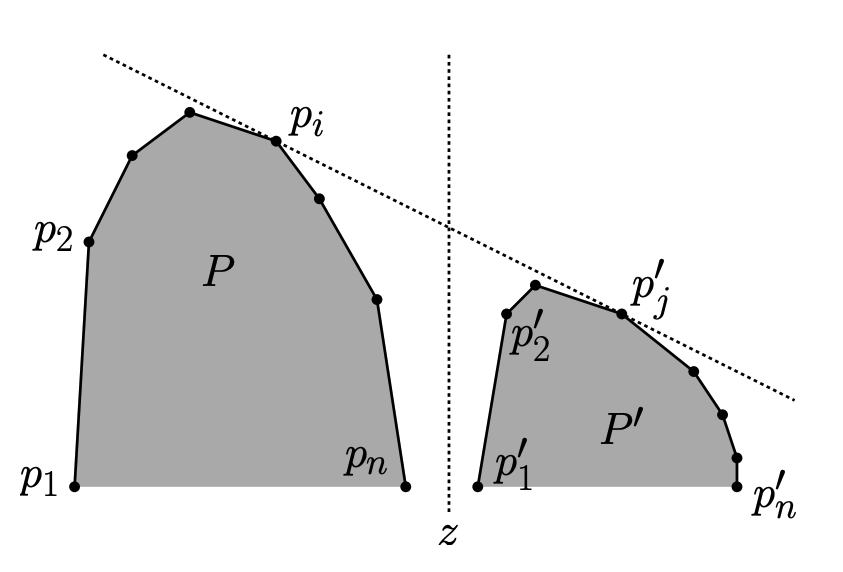
\includegraphics[width=0.5\textwidth]{tangents}
    \caption{Problem 1: Computing the upper tangent of two hulls}
\end{figure}

Present a $\Theta(\log n)$-time algorithm which, given $P$ and $P'$, computes the two
points $p_i \in P$ and $p_j' \in P'$ such that their common support line passes
through these two points.

Briefly justify your algorithm's correctness and derive its running time.  ({\bf
Hint:} The correctness proof involves a case analysis.  Please be careful, a
poorly drawn figure may lead to an incorrect hypothesis.)

\paragraph{Answer}

\todo{replace this TODO with your answer}
%%%%%%%%%%%%%%%%%%%%%%%%%%%%%%%%%%%%%%%%%%%%%%%%%%%%%%%%%%%%%%%%%%%%%%%%%%%%%%

%%%%%%%%%%%%%%%%%%%%%%%%%%%%%%%%%%%%%%%%%%%%%%%%%%%%%%%%%%%%%%%%%%%%%%%%%%%%%%
\collab{\todo{}}
\nextprob{Pareto Set}

Consider a set $P = \{p_1, \ldots, p_n \}$ of points in the plane, where $p_i =
(p_i^{(1)}, p_i^{(2)})$. A \emph{Pareto set} for $P$, denoted $\pareto{P}$, (named after
the Italian engineer and economist Vilfredo Pareto), is a subset of
points~$p_i$ such that there is no $p_j \in P$ with $j \neq i$ such that $p_j^{(1)}
\geq p_i^{(1)}$ and
$p_j^{(2)} \geq p_i^{(2)}$.  That is, each point of $\pareto{P}$ has the property that
there is no point of $P$ that is both to the right and above it.

\begin{figure}[h]
    \centering
    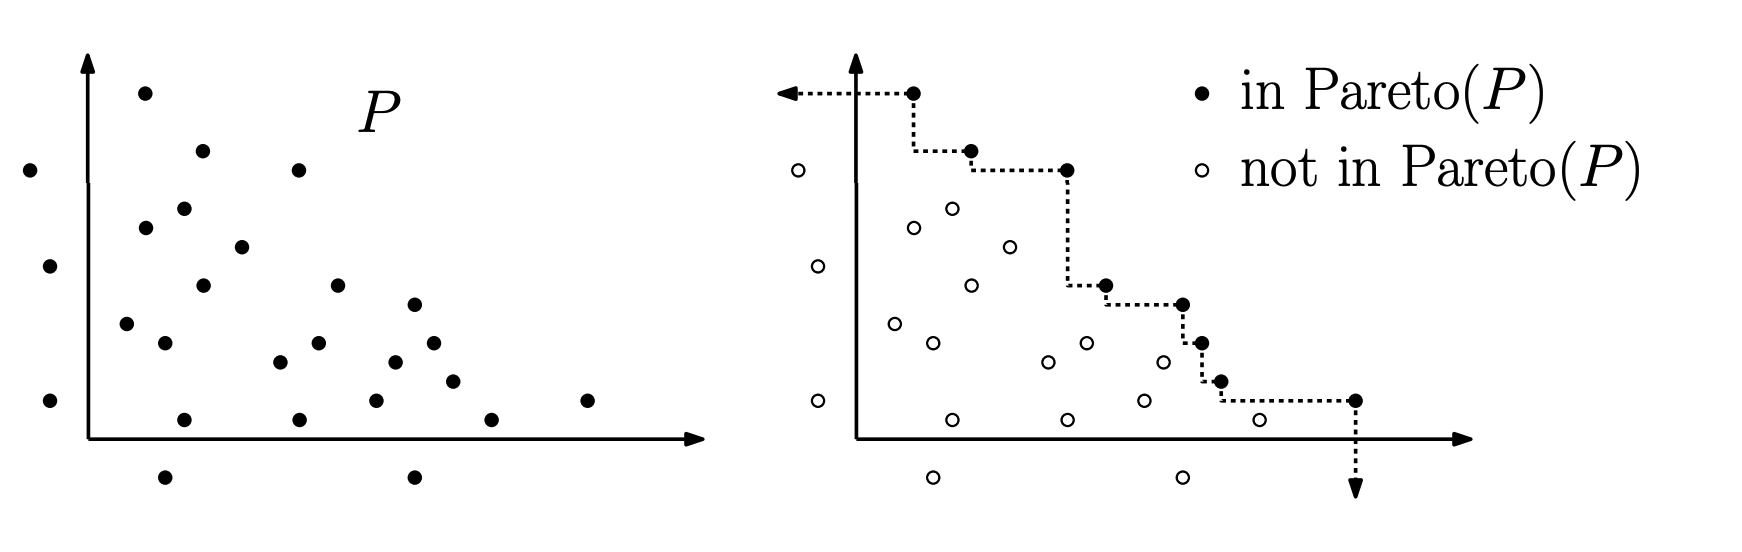
\includegraphics[width=0.75\textwidth]{pareto}
    \caption{Problem 2: Pareto set}
\end{figure}

Pareto sets and convex hulls in the plane are similar in many respects.  In
this problem we will explore some of these connections.

\begin{enumerate}

    \item A point $p$ lies on the convex hull of a set $P$ if and only if there is
        a line passing though $p$ such that all the points of $P$ lie on one side of
        this line.  Provide an analogous assertion for the points of $\pareto{P}$ in
        terms of a different shape.

        \paragraph{Answer}
        \todo{replace this TODO with your ans}

    \item Devise an analogue of Graham's convex-hull algorithm for computing
        \pareto{P} in $O(n \log n)$ time.  Briefly justify your algorithm's correctness
        and derive its running time.  (You do not need to explain the algorithm ``from
        scratch'', that is, you can explain with modifications would be made to Grahm's
        algorithm.)

        \paragraph{Answer}
        \todo{replace this TODO with your ans}

    \item Devise an analogue of the Jarvis march algorithm for computing
        $\pareto{P}$ in $O(h \cdot n)$ time, where $h$ is the cardinality of
        $\pareto{P}$.  (As with the previous part, you can just explain the differences
        with Jarvis's algorithm.)

        \paragraph{Answer}
        \todo{replace this TODO with your ans}

    \item Devise an algorithm for computing $\pareto{P}$ in $O(n
        \log h)$ time, where $h$ is the cardinality of $\pareto{P}$.

        \paragraph{Answer}
        \todo{replace this TODO with your ans}

\end{enumerate}
%%%%%%%%%%%%%%%%%%%%%%%%%%%%%%%%%%%%%%%%%%%%%%%%%%%%%%%%%%%%%%%%%%%%%%%%%%%%%%


\end{document}

%%%%%%%%%%%%%%%%%%%%%%%%%%%%%%%%%%%%%%%%%%%%%%%%%%%%%%%%%%%%%%%%%%%%%%%%%%%%%%
\collab{\todo{}}
\nextprob{NAME}

PROBLEM

\paragraph{Answer}

\todo{replace this TODO with your answer}
%%%%%%%%%%%%%%%%%%%%%%%%%%%%%%%%%%%%%%%%%%%%%%%%%%%%%%%%%%%%%%%%%%%%%%%%%%%%%%


